\documentclass[aspectratio=169,11pt]{beamer}
\usepackage[T1]{fontenc}
\usepackage{lmodern,booktabs,array,tikz,pgfplots,amsmath}
\usetikzlibrary{arrows.meta,positioning,calc}
\pgfplotsset{compat=1.18}
\definecolor{Ink}{HTML}{17324D}
\definecolor{Teal}{HTML}{007F7B}
\definecolor{Rust}{HTML}{B5533C}
\definecolor{Gray}{HTML}{657483}
\definecolor{Soft}{HTML}{EEF3F6}
\setbeamercolor{normal text}{fg=Ink,bg=white}
\setbeamercolor{frametitle}{fg=Ink}
\setbeamercolor{structure}{fg=Teal}
\setbeamercolor{block title}{fg=white,bg=Teal}
\setbeamercolor{block body}{fg=Ink,bg=Soft}
\setbeamercolor{alerted text}{fg=Rust}
\setbeamertemplate{navigation symbols}{}
\setbeamertemplate{itemize items}[circle]
\setbeamersize{text margin left=9mm,text margin right=9mm}
\setbeamerfont{frametitle}{size=\large,series=\bfseries}
\setbeamertemplate{footline}{\hspace{9mm}\scriptsize Reproducing SPO on GSM8K: a tutorial\hfill\insertframenumber/\inserttotalframenumber\hspace{9mm}\vspace{3mm}}
\newcommand{\source}[1]{\vfill{\scriptsize\color{Gray}#1\par}}
\hypersetup{pdftitle={Reproducing SPO on GSM8K: a tutorial},pdfauthor={Alex Towell}}
\title{Reproducing Segment Policy Optimization on GSM8K}
\subtitle{A tutorial on RL for language models, told through one audited reproduction}
\author{Alex Towell}
\date{October 2026 \quad\textcolor{Gray}{Paper: Guo, Xu, Liu, Ye, Qiu, arXiv:2505.23564. Code: AIFrameResearch/SPO.}}
\begin{document}

\begin{frame}[plain]
\titlepage
\vfill
\begin{block}{In one sentence}
Rerunning the authors' code on one A100 took a math model from 39.8\% to 58.2\% on GSM8K,
a little above the paper's 56.7\%, with the comparison point fixed before training.
\end{block}
\end{frame}

\begin{frame}[t]
\frametitle{Reproduce a known result before trusting a new one.}
\begin{columns}[T,onlytextwidth]
\begin{column}{.48\textwidth}
\textbf{The situation.} We want to train a model with reinforcement learning (RL) on a task
where nobody has published numbers. If it fails, we will not know whether the method, the
code, or the measurement is at fault.
\medskip

\textbf{The move.} First rerun a published RL result whose answers can be checked
automatically. Every part of the pipeline gets tested against a known target.
\end{column}
\begin{column}{.48\textwidth}
\begin{block}{What a reproduction buys}
\begin{itemize}
\item A tested evaluator (score the authors' released model).
\item A tested training loop (retrain and recover the score).
\item A list of the places where things silently go wrong.
\end{itemize}
\end{block}
\end{column}
\end{columns}
\source{This deck follows the written walkthrough at queelius.github.io/spo-gsm8k-reproduction; every number has a receipt in the repository's docs/evidence folder.}
\end{frame}

\begin{frame}[t]
\frametitle{The task: grade-school math with a checkable final answer.}
\begin{columns}[T,onlytextwidth]
\begin{column}{.56\textwidth}
\small
\textbf{Question (GSM8K test, item 0).} Janet's ducks lay 16 eggs per day. She eats three for
breakfast every morning and bakes muffins for her friends every day with four. She sells the
remainder at the farmers' market daily for \$2 per fresh duck egg. How much in dollars does she
make every day at the farmers' market?
\medskip

\textbf{Gold solution.}\\
Janet sells $16-3-4=9$ duck eggs a day.\\
She makes $9\times 2=18$ dollars every day.\\
\texttt{\#\#\#\# 18}
\end{column}
\begin{column}{.40\textwidth}
\begin{block}{How an answer is scored}
Take the text after the last \texttt{\#\#\#\#}, strip commas, compare as a string to the gold
answer. Correct $\to$ reward $1$; wrong $\to 0$; no marker or cut off $\to -1$.
\end{block}
\medskip
\textbf{Splits used:} 7,100 train / 373 validation / 1,319 test.\\[1mm]
\textbf{Metric:} mean pass@1 over 16 sampled answers per test question (21,104 answers).
\end{column}
\end{columns}
\source{Cobbe et al. 2021 (GSM8K). The checker is the authors' own; it is exact string matching, so 1600 against 1,600 scores zero.}
\end{frame}

\begin{frame}[t]
\frametitle{RL for a language model: sample, score, update.}
\begin{center}
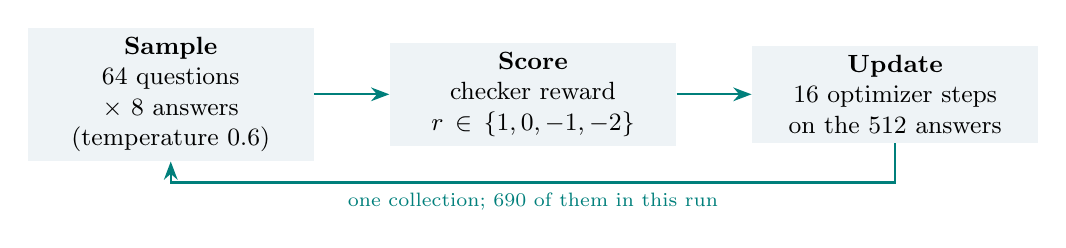
\begin{tikzpicture}[every node/.style={font=\small,align=center},>=Stealth]
\node[fill=Soft,text width=3.4cm,minimum height=1.2cm] (a) at (0,0) {\textbf{Sample}\\64 questions $\times$ 8 answers\\(temperature 0.6)};
\node[fill=Soft,text width=3.4cm,minimum height=1.2cm] (b) at (4.6,0) {\textbf{Score}\\checker reward\\$r\in\{1,0,-1,-2\}$};
\node[fill=Soft,text width=3.4cm,minimum height=1.2cm] (c) at (9.2,0) {\textbf{Update}\\16 optimizer steps\\on the 512 answers};
\draw[->,thick,Teal] (a)--(b); \draw[->,thick,Teal] (b)--(c);
\draw[->,thick,Teal] (c.south) -- ++(0,-.5) -| (a.south) node[pos=.25,below,font=\scriptsize\color{Gray}]{one collection; 690 of them in this run};
\end{tikzpicture}
\end{center}
\begin{columns}[T,onlytextwidth]
\begin{column}{.48\textwidth}
\textbf{Policy} $\pi_\theta(y\mid x)$: the model's probability of answer $y$ to prompt $x$,
one token at a time.\\[1mm]
\textbf{Advantage} $A_t$: how much better token $t$ was than expected. Positive advantage
raises its probability.
\end{column}
\begin{column}{.48\textwidth}
\textbf{PPO clipping.} With ratio $\rho_t=\pi_\theta/\pi_{\text{old}}$, the loss is
$-\min(\rho_t A_t,\ \mathrm{clip}(\rho_t,0.8,1.2)\,A_t)$, so one update cannot move far
from the sampler. A small KL term ($10^{-4}$) keeps the policy near the starting model.
\end{column}
\end{columns}
\source{Schulman et al. 2017 (PPO). The guard that zeroes a batch whose mean ratio exceeds 10 returns on slide 10.}
\end{frame}

\begin{frame}[t]
\frametitle{The problem: one number at the end has to pay 100 to 300 tokens.}
\begin{center}
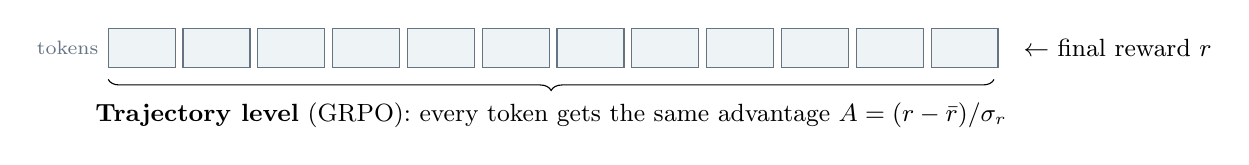
\begin{tikzpicture}[>=Stealth,font=\small]
\foreach \i in {0,...,11}{\draw[fill=Soft,draw=Gray] (\i*0.95,0) rectangle ++(0.85,0.5);}
\node[right] at (11.5,0.25) {$\leftarrow$ final reward $r$};
\node[left,font=\scriptsize\color{Gray}] at (0,0.25) {tokens};
\draw[decorate,decoration={brace,mirror,amplitude=4pt}] (0,-0.15) -- (11.25,-0.15) node[midway,below=5pt]{\textbf{Trajectory level} (GRPO): every token gets the same advantage $A=(r-\bar r)/\sigma_r$};
\end{tikzpicture}
\end{center}
\vspace{-1mm}
\begin{columns}[T,onlytextwidth]
\begin{column}{.31\textwidth}
\textbf{Trajectory level}\\[1mm]
Cheap, no critic. But a wrong answer with a good first half gets no internal distinction,
and a group of 8 that all agree gives zero signal.
\end{column}
\begin{column}{.31\textwidth}
\textbf{Token level} (PPO + critic)\\[1mm]
A value for every token, from a second model trained on noisy targets. Most informative in
principle; the estimates are often inaccurate in practice.
\end{column}
\begin{column}{.31\textwidth}
\textbf{Segment level} (SPO)\\[1mm]
Cut the answer at a few points, estimate the value at each cut by sampling, give each
segment one advantage. VinePPO does this at every line; SPO cuts fewer, smarter.
\end{column}
\end{columns}
\source{Shao et al. 2024 (GRPO); Kazemnejad et al. 2024 (VinePPO). The SPO code base is a fork of VinePPO's.}
\end{frame}

\begin{frame}[t]
\frametitle{SPO-chain: cut where the model was unsure, value each cut by sampling.}
\begin{center}
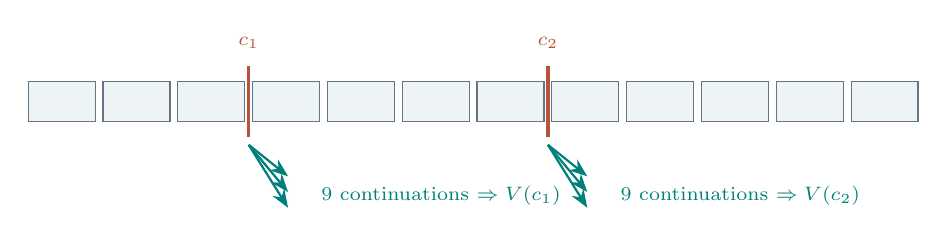
\begin{tikzpicture}[>=Stealth,font=\small]
\foreach \i in {0,...,11}{\draw[fill=Soft,draw=Gray] (\i*0.95,0) rectangle ++(0.85,0.5);}
\foreach \i in {3,7}{\draw[very thick,Rust] (\i*0.95-0.05,-0.2) -- ++(0,0.9);}
\node[Rust,font=\scriptsize] at (3*0.95-0.05,1.0) {$c_1$};
\node[Rust,font=\scriptsize] at (7*0.95-0.05,1.0) {$c_2$};
\foreach \k in {0,1,2}{\draw[->,Teal,thick] (3*0.95-0.05,-0.3) -- ++(0.5,-0.4-\k*0.2);}
\node[Teal,font=\scriptsize,anchor=west] at (3.6,-0.95) {9 continuations $\Rightarrow V(c_1)$};
\foreach \k in {0,1,2}{\draw[->,Teal,thick] (7*0.95-0.05,-0.3) -- ++(0.5,-0.4-\k*0.2);}
\node[Teal,font=\scriptsize,anchor=west] at (7.4,-0.95) {9 continuations $\Rightarrow V(c_2)$};
\end{tikzpicture}
\end{center}
\small
\begin{columns}[T,onlytextwidth]
\begin{column}{.48\textwidth}
\textbf{1. Partition.} Mark tokens the sampler gave $p_t<0.9$; shift each mark back one
token; keep every 5th mark (the \emph{interval}). About 3 cutpoints per answer here.
\medskip

\textbf{2. Value at a cut.} $V(c_k)=\frac19\sum_{j=1}^{9} r(x,\,y_{\le c_k}\oplus z_j)$:
the chance of finishing correctly from this prefix. No critic.
\end{column}
\begin{column}{.48\textwidth}
\textbf{3. Segment advantage.} $A_k=V(c_k)-V(c_{k-1})$ for the tokens between two cuts;
the last segment gets $r-V(c_K)$; the first gets 0 in the public code.
\medskip

\textbf{4. Update.} Mask out confident tokens ($p_t>0.9$), whiten the advantages, then the
PPO-clip step of the previous slide.
\end{column}
\end{columns}
\source{As implemented at the pinned commit. Cost: about 14,600 continuation samples per 512 answers.}
\end{frame}

\begin{frame}[t]
\frametitle{What the paper reports, and what we set out to match.}
\begin{columns}[T,onlytextwidth]
\begin{column}{.52\textwidth}
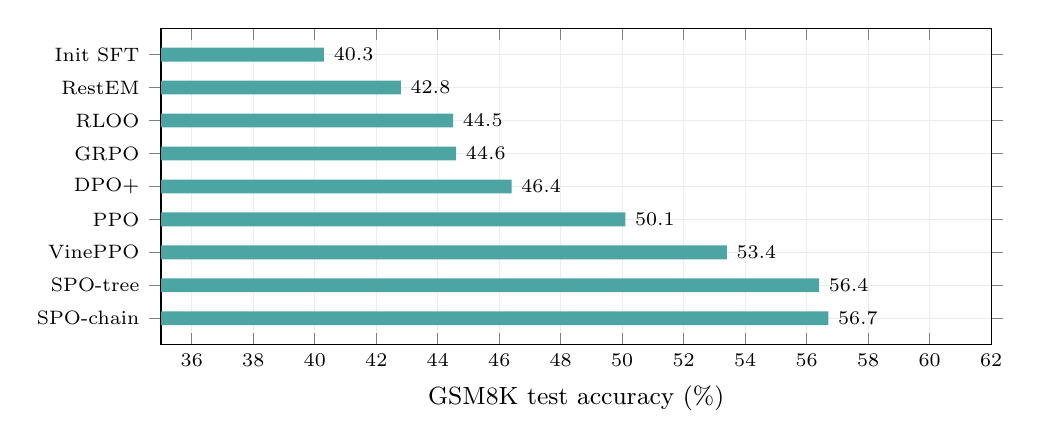
\begin{tikzpicture}
\begin{axis}[xbar,width=\linewidth,height=5.6cm,xmin=35,xmax=62,bar width=5pt,
ytick=data,symbolic y coords={Init SFT,RestEM,RLOO,GRPO,DPO+,PPO,VinePPO,SPO-tree,SPO-chain},
y dir=reverse,tick label style={font=\scriptsize},xlabel={GSM8K test accuracy (\%)},label style={font=\small},
nodes near coords,nodes near coords style={font=\scriptsize},grid=major,grid style={gray!15}]
\addplot[fill=Teal!70,draw=none] coordinates {(40.3,Init SFT)(42.8,RestEM)(44.5,RLOO)(44.6,GRPO)(46.4,DPO+)(50.1,PPO)(53.4,VinePPO)(56.4,SPO-tree)(56.7,SPO-chain)};
\end{axis}
\end{tikzpicture}
\end{column}
\begin{column}{.45\textwidth}
\textbf{Setting.} RhoMath 1.1B, already supervised-fine-tuned on GSM8K, then RL.
\medskip

\textbf{Target.} SPO-chain, 56.7\%, which the audit traced to checkpoint 690 of a
1,000-iteration schedule in the authors' logs.
\medskip

\textbf{Caveat the paper's own caption states:} the baseline bars are inherited from the
VinePPO paper, not rerun.
\end{column}
\end{columns}
\source{Figure 3 of the official README (RhoMath 1.1B, GSM8K). Values read from the figure; 56.7 confirmed from the authors' W\&B log (0.56724).}
\end{frame}

\begin{frame}[t]
\frametitle{What we ran: the authors' code, one GPU, a comparison point fixed in advance.}
\small
\begin{columns}[T,onlytextwidth]
\begin{column}{.50\textwidth}
\begin{tabular}{@{}>{\raggedright\arraybackslash}p{.2\linewidth}>{\raggedright\arraybackslash}p{.76\linewidth}@{}}
\toprule
Code & AIFrameResearch/SPO at commit 6c5f947, unmodified\\
Start & realtreetune/rho-1b-sft-GSM8K (the authors' SFT model)\\
Recipe & recovered from the authors' logs: seed 42, LR $10^{-6}$, 64 questions $\times$ 8 answers, 9 continuations, interval 5\\
Hardware & one A100 40 GB, about 51 hours\\
Endpoint & collection 690 / update 11,040, declared before training\\
\bottomrule
\end{tabular}
\end{column}
\begin{column}{.46\textwidth}
\begin{block}{Why fix the endpoint first}
The paper's number is one checkpoint of a long schedule, and nothing records why that one.
Picking our best test checkpoint afterwards would make the comparison meaningless.
\end{block}
\begin{block}{Two separate checks}
Scoring the authors' released model (56.69\% here vs 56.72\% in their log) tests the
\emph{evaluator}. Training our own model tests \emph{learning}. Only the second is the result.
\end{block}
\end{column}
\end{columns}
\source{docs/protocol-audit.md; docs/evidence/author-reference-*.json; environment lock env/requirements-spo-6c5f947.txt.}
\end{frame}

\begin{frame}[t]
\frametitle{Result: our training recovered the paper's level, at a pre-declared endpoint.}
\begin{columns}[T,onlytextwidth]
\begin{column}{.61\textwidth}
\begin{tikzpicture}
\begin{axis}[width=\linewidth,height=4.9cm,xmin=0,xmax=11600,ymin=35,ymax=65,
xlabel={Optimizer updates},ylabel={Test mean pass@1 (\%)},
scaled x ticks=false,xtick={0,4000,8000,11040},xticklabels={0,4k,8k,11k},
ytick={35,40,45,50,55,60,65},tick label style={font=\scriptsize},
label style={font=\small},grid=major,grid style={gray!15},
legend style={font=\scriptsize,at={(.97,.08)},anchor=south east,draw=none,fill=white}]
\addplot[Teal,thick] table[x=updates,y=test_percent,col sep=comma]{learning-curve.csv};
\addlegendentry{Our run (70 scheduled tests, all regraded)}
\addplot[Gray,dashed,thick] coordinates {(0,56.7)(11600,56.7)};
\addlegendentry{Paper: 56.7\%}
\addplot[only marks,mark=*,mark size=2.8pt,Rust] coordinates {(11040,58.1927596664)};
\addlegendentry{Fixed endpoint: 58.19\%}
\end{axis}
\end{tikzpicture}
\end{column}
\begin{column}{.36\textwidth}
\small
\begin{tabular}{@{}lr@{}}
\toprule
Matched SFT start & 39.77\%\\
Paper & 56.70\%\\
\textbf{Ours, endpoint} & \textbf{58.19\%}\\
Ours, best intermediate & 58.32\%\\
\bottomrule
\end{tabular}
\medskip

12,281 of 21,104 answers correct.\\[1mm]
\textbf{Gain over the matched start: +18.4 points.}\\[1mm]
One seed, one task: a performance-level reproduction, not statistical equivalence.
\end{column}
\end{columns}
\source{docs/evidence/final690-audit-20261014.json; slides/learning-curve.csv with curve-provenance.json mapping each point to its receipt and hash.}
\end{frame}

\begin{frame}[t]
\frametitle{The first attempt collapsed; the diagnosis is the most useful part.}
\small
\begin{columns}[T,onlytextwidth]
\begin{column}{.50\textwidth}
\textbf{What we saw.} Test accuracy rose to 50.5\% at 4,336 updates, fell to
\alert{22.2\%} at 7,856, and the process crashed at step 7,995.
\medskip

\textbf{Was it the scorer?} No: an independent CPU regrade of 66,048 saved answers matched
every metric. The model really got worse (96 questions went from 16/16 to 0/16).
\medskip

\textbf{Why the crash?} Four batches in a row hit the PPO ratio guard (mean ratios 95, 37,
153, 10), were zeroed, and the BF16 optimizer asserted on a gradient norm of exactly zero.
\end{column}
\begin{column}{.46\textwidth}
\begin{block}{The input mismatch}
Generation requests started with the BOS token; the training-side tokenizer omitted it.
Answers were sampled under one input and scored under another. Adding BOS shifted the
late model's log-likelihood by $+54$ nats on average ($-0.1$ for the SFT model).
\end{block}
\medskip
\textbf{Fixes, each isolated and hash-pinned:} a BOS adapter, a finite-zero-norm adapter,
a fixed-endpoint hook; then a restart from the original SFT weights.
\end{column}
\end{columns}
\source{docs/diagnosis-and-restart-20261012.md. The mismatch is a supported hypothesis for the decline, not a demonstrated cause: no ablation was run.}
\end{frame}

\begin{frame}[t]
\frametitle{Deviations from the paper, stated plainly.}
\begin{tabular}{@{}>{\raggedright\arraybackslash}p{.30\textwidth}>{\raggedright\arraybackslash}p{.64\textwidth}@{}}
\toprule
Item & What differs and why\\
\midrule
Evaluation top-p & Paper says 0.9; the evaluation template omits the argument, so 1.0 applies, in the authors' historical pipeline too. Kept at 1.0 for an exact reference comparison.\\[1mm]
BOS token & Prepended during training by our adapter; the public source has it commented out. Whether the authors' run added it is unknown.\\[1mm]
Zero gradient norm & Accepted as finite (DeepSpeed asserts $>0$); NaN and Inf still rejected.\\[1mm]
Config vs code & Recipe recovered from the authors' logs, not a recorded git revision; README defaults differ from the historical run.\\[1mm]
Scope & One seed, one task, no GRPO control, checkpoint copies on the same filesystem.\\
\bottomrule
\end{tabular}
\source{Full list with receipts: docs/protocol-audit.md and docs/final-result-20261014.md.}
\end{frame}

\begin{frame}[t]
\frametitle{Lessons that transfer to any RL experiment.}
\small
\begin{columns}[T,onlytextwidth]
\begin{column}{.48\textwidth}
\begin{itemize}
\item \textbf{Fix the comparison point before training}, or you will select the best test checkpoint without noticing.
\item \textbf{Score a known model first.} Seven minutes on the authors' checkpoint separated evaluator bugs from training bugs for a week.
\item \textbf{Report the gain from a matched baseline} under one scoring rule: 39.8 $\to$ 58.2 is the result, not 58.2.
\end{itemize}
\end{column}
\begin{column}{.48\textwidth}
\begin{itemize}
\item \textbf{Check that the tokens you reward are the tokens you scored}, BOS included.
\item \textbf{Regrade saved answers independently} of the training code; it is cheap and rules out scoring bugs in minutes.
\item \textbf{Read the safeguards.} A guard that ``skips'' a batch produced a zero gradient and crashed the optimizer.
\item \textbf{Preserve failures.} The collapsed run's artifacts made the diagnosis possible.
\end{itemize}
\end{column}
\end{columns}
\source{Every item above corresponds to a receipt in docs/evidence; the walkthrough's section 11 lists them.}
\end{frame}

\begin{frame}[t]
\frametitle{Reproduce it yourself.}
\small
\begin{enumerate}
\item \textbf{Environment.} Python 3.10 from \texttt{env/requirements-spo-6c5f947.txt}; clone AIFrameResearch/SPO at commit 6c5f947 and leave it unmodified.
\item \textbf{Assets.} Dataset archive and the two Hugging Face models at the pinned revisions; verify the hashes in \texttt{docs/evidence/}.
\item \textbf{Reference checks.} Run the recorded argv in \texttt{author-reference-command.json}; regrade; expect 0.5669 and 0.3977.
\item \textbf{Train.} \texttt{code/launch\_bos\_only.py --configs fresh\_bos\_only.jsonnet run\_iteration\_loop} with the environment variables in \texttt{restart-20261012.json}; run the CPU tests first.
\item \textbf{Watch, regrade, preserve.} \texttt{code/review\_monitor.py}; regrade each scheduled evaluation; after the endpoint hook, copy and hash the 690 checkpoint.
\end{enumerate}
\source{Copy commands from the receipts rather than retyping them; the walkthrough's section 12 names each one. Repository: github.com/queelius/spo-gsm8k-reproduction (MIT; the authors' code is MIT).}
\end{frame}

\appendix
\begin{frame}[t]
\frametitle{Appendix: glossary.}
\small
\begin{tabular}{@{}>{\raggedright\arraybackslash}p{.24\textwidth}>{\raggedright\arraybackslash}p{.70\textwidth}@{}}
\toprule
Advantage & value achieved minus value expected; the per-token learning signal.\\
BOS / EOS & beginning- and end-of-sequence tokens a tokenizer may add.\\
Collection & 64 questions $\times$ 8 answers plus Monte Carlo sampling, then 16 updates.\\
Cutpoint & a response position chosen for a value estimate.\\
GRPO & group-normalised trajectory-level advantages; no critic.\\
Mean pass@1 & mean over questions of the fraction of 16 samples that are correct.\\
Monte Carlo value & mean reward of sampled continuations from a prefix.\\
PPO ratio & new-policy over sampling-policy probability of a token.\\
Probability mask & exclude tokens the sampler was already sure about ($p_t>0.9$).\\
Segment & the tokens between two cutpoints.\\
SFT & supervised fine-tuning; the starting model was SFT'd on GSM8K.\\
\bottomrule
\end{tabular}
\end{frame}
\end{document}
